\chapter{Ultrafast Carrier Dynamics of (6,5) After Resonant E$_{22}$ Pumping}

\section{Overview}

\section{Experimental Results}

\begin{figure}[H]
	\centering
	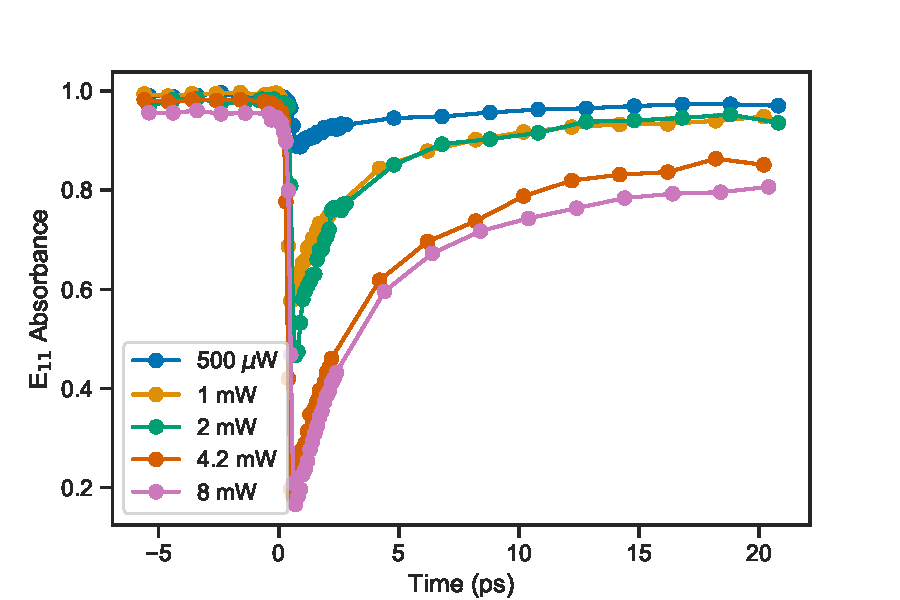
\includegraphics[scale=0.75]{images/chapter_my_data/absorbance_dynamics_E11}
	\caption{Data}
\end{figure}

\begin{figure}[H]
	\centering
	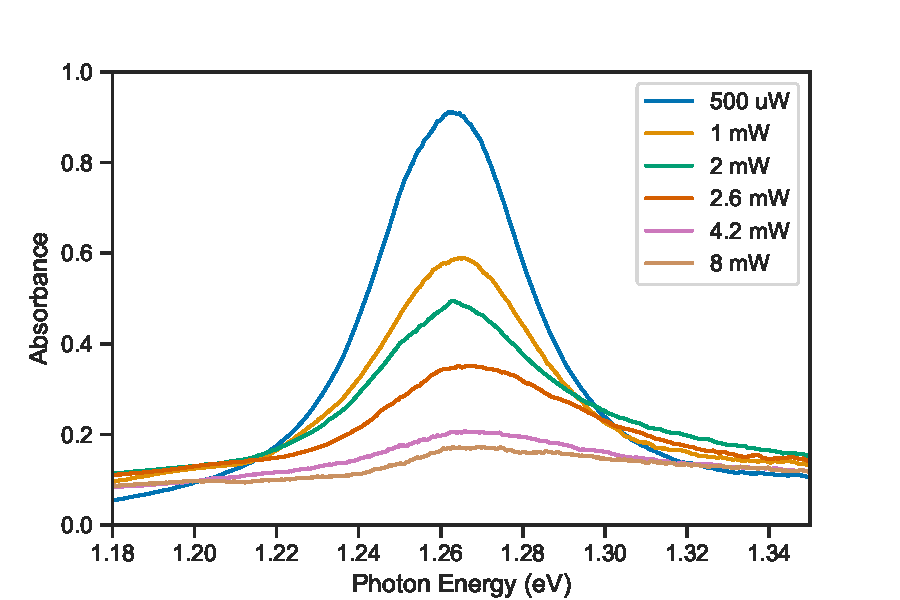
\includegraphics[scale=0.75]{images/chapter_my_data/peak_abs_vs_pump}
	\caption{Data}
\end{figure}

\begin{figure}[H]
	\centering
	\begin{subfigure}{0.46\textwidth}
		\centering
		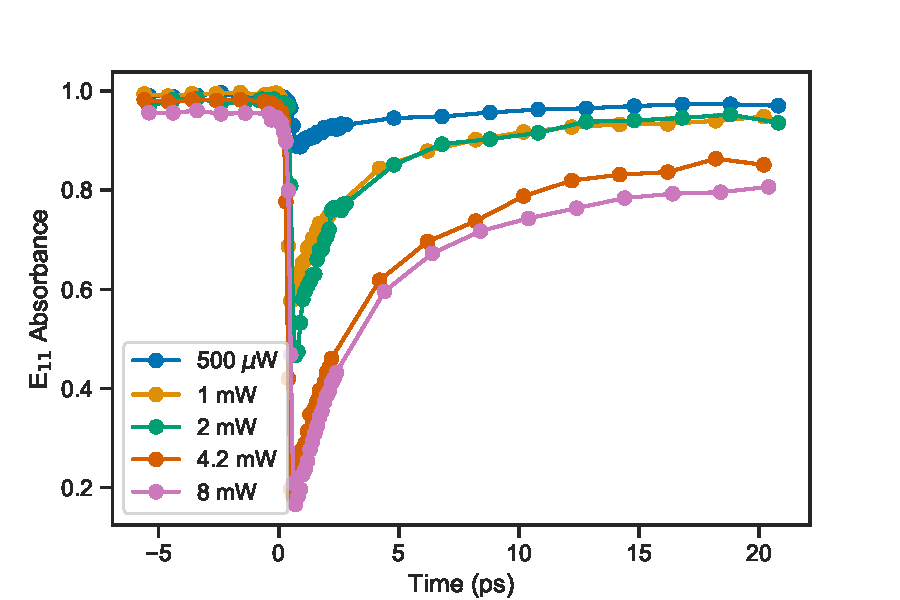
\includegraphics[scale=0.55]{images/chapter_my_data/absorbance_dynamics_E11}
		\caption{A}
	\end{subfigure}
	\qquad
	\centering
	\begin{subfigure}{0.46\textwidth}
		\centering
		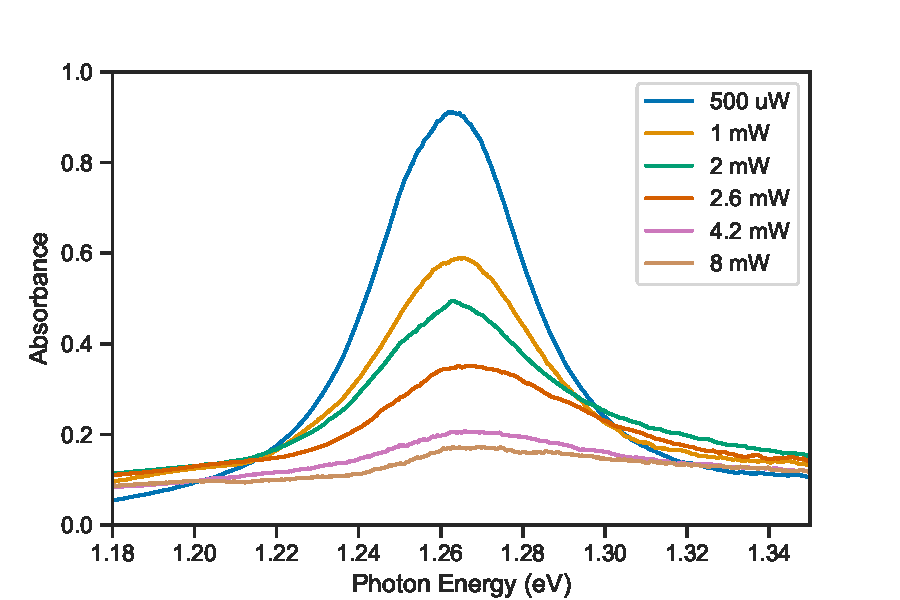
\includegraphics[scale=0.55]{images/chapter_my_data/peak_abs_vs_pump}
		\caption{B}
	\end{subfigure}
	\caption{Data}
\end{figure}


\section{Data Analysis}
\begin{figure}[H]
	\centering
	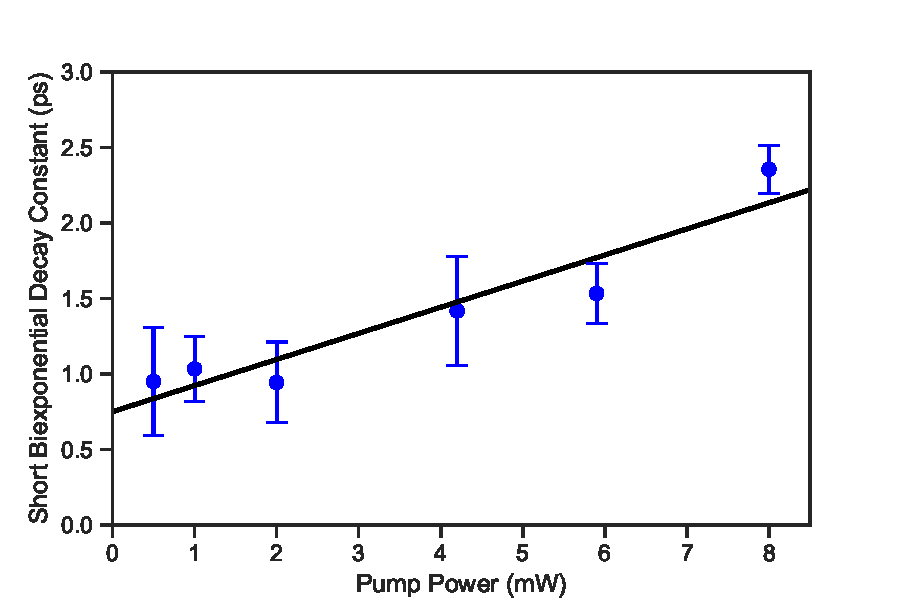
\includegraphics[scale=0.8]{images/chapter_my_data/shorter_biexpconst_fit}
	\caption{Data}
\end{figure}

\section{Discussion}
Exciton-Exciton annihilation supposedly efficient \cite{murakami2009existence}


\section{Conclusions}